\graphicspath{{Images/untetheredWalker/}}

\chapter{Miniature Untethered Underwater Walking Robot}
\label{chap:untetheredWalker}
Current soft actuators rely on additional hardware such as pumps, high voltage supplies, light generation sources and magnetic field generators for their operation. 
% Assembling these actuators results in bulky robotic systems, although the body of the soft robot itself may remain miniaturized. 
These components resist miniaturization and embedding them into small-scale soft robots would be challenging. This limits their mobile applications where the entire system needs to be untethered especially in hyper-redundant robots where a high number of actuators are needed. Here, we introduce miniature and untethered robots made of soft voxel actuators (SVAs) -- an active voxel using stimuli-responsive hydrogels actuated by electrical currents through Joule heating. SVAs weighing only 100\,mg require small footprint microcontrollers for their operation which can be embedded in the robotic system. We have demonstrated the advantages of hydrogel-based SVAs through a hyper-redundant manipulator with 16 actuators and an untethered miniature robot for underwater mobile applications.
\section{Background}
Inspired by biology, soft robot developers try to utilize the advantages inherent in soft, compliant matter to achieve safer interactions around humans or more robust locomotion and manipulation in unstructured environments~\cite{martinez2013robotic,laschi2012soft,tolley2014resilient,bilodeau2015monolithic}.  
Soft pneumatic actuators (SPAs)~\cite{Gorissen2017, branyan2017soft} are the most widely used category in soft robotics. SPAs use passive materials such as silicone and rely on rigid components such as motors and pumps that are difficult to downscale and therefore, manufacturing small-scale soft actuators which have applications as envisioned by \cite{hines2017soft} has remained a bottleneck in the development of miniaturized soft robots \cite{majidi2019soft}. 

Stimuli-responsive, soft materials have shown promise in solving some of these challenges \cite{steele2018stimuli, stuart2010emerging,white2013advances}. The changes in the stress/strain distribution in these materials in reaction to variations in pH, temperature, electric field, magnetic field, and light results in motions such as bending, twisting, or elongation. However, the equipment needed to create variable stimuli such as structured light \cite{palagi2016structured} or magnetic field \cite{Kim2018} are still bulky. Temperature responsive hydrogels, by contrast, can be stimulated electrically using Joule heating \cite{yu2013electronically}. The electrical stimulation can be confined to small regions making it possible to create more precise motions \cite{richter2009optoelectrothermic}. We have previously reported solving some of the challenges associated with temperature responsive poly(N-isopropylacrylamide) (PNIPAAm) based hydrogels such as their slow response and tuning their mechanical properties. We have also introduced blocks called soft voxel actuators (SVAs), which are electrically activated by Joule heaters \cite{Khodambashi2021}. In this communication, we demonstrate how SVAs support the development of soft robots which are miniature and untethered --two key characteristics that are challenging to realize with pneumatic soft actuators. We introduce a miniature completely untethered robot for underwater applications which weighs only 20\,g including battery and electronics as shown in Fig.~\ref{fig:concept}. We also demonstrate the use of SVAs to build a miniature continuum manipulator with hyper-redundant DOFs as shown in Fig.~\ref{fig:treajectory}A. This manipulator is 10$\times$ 40 $\times$ 4.5\,mm$^3$ and has 16 actuators. 

\begin{figure}[!t]
\centering
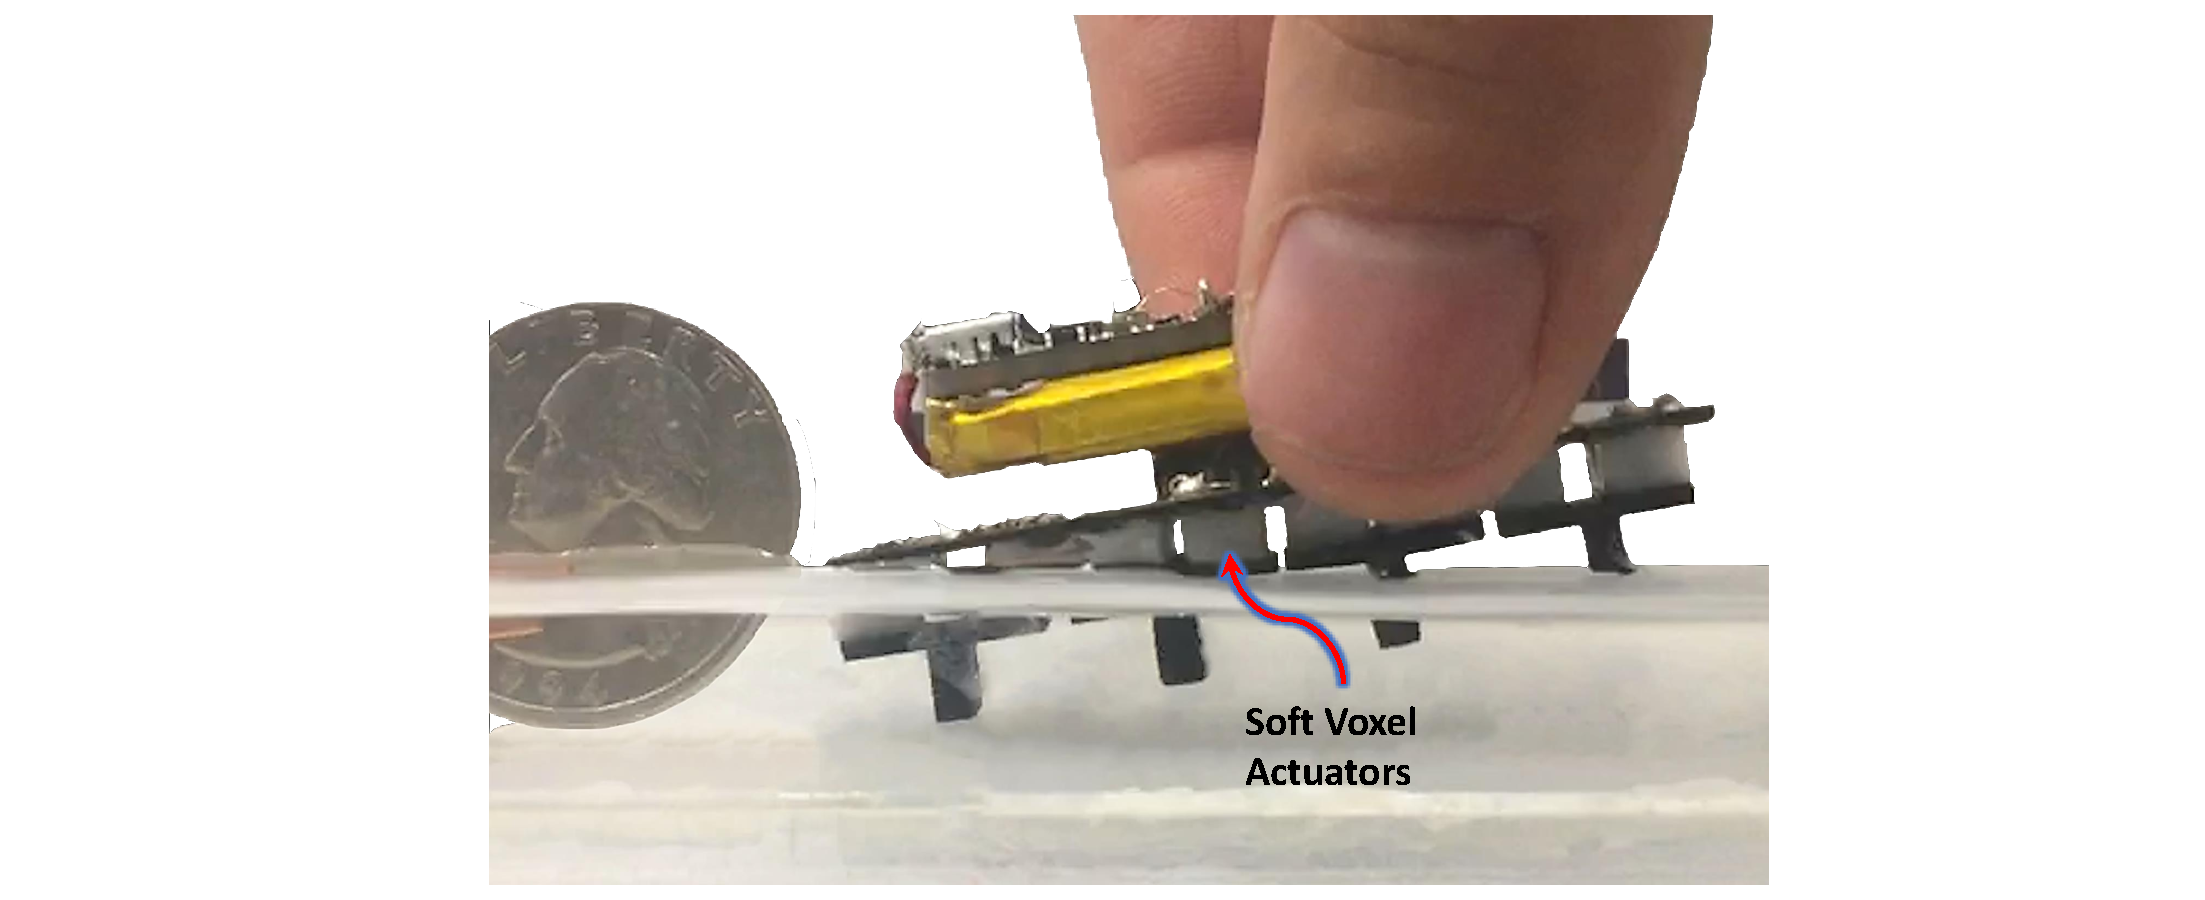
\includegraphics[width=0.7\textwidth]{Fig1.pdf}
    \caption[Untethered miniature underwater walking robot]{An untethered miniature underwater walking robot using 8 SVAs is made which weighs only 20\,g including battery and electronics.}
    \label{fig:concept}
\end{figure}
\begin{figure*}[!t]
      \centering
      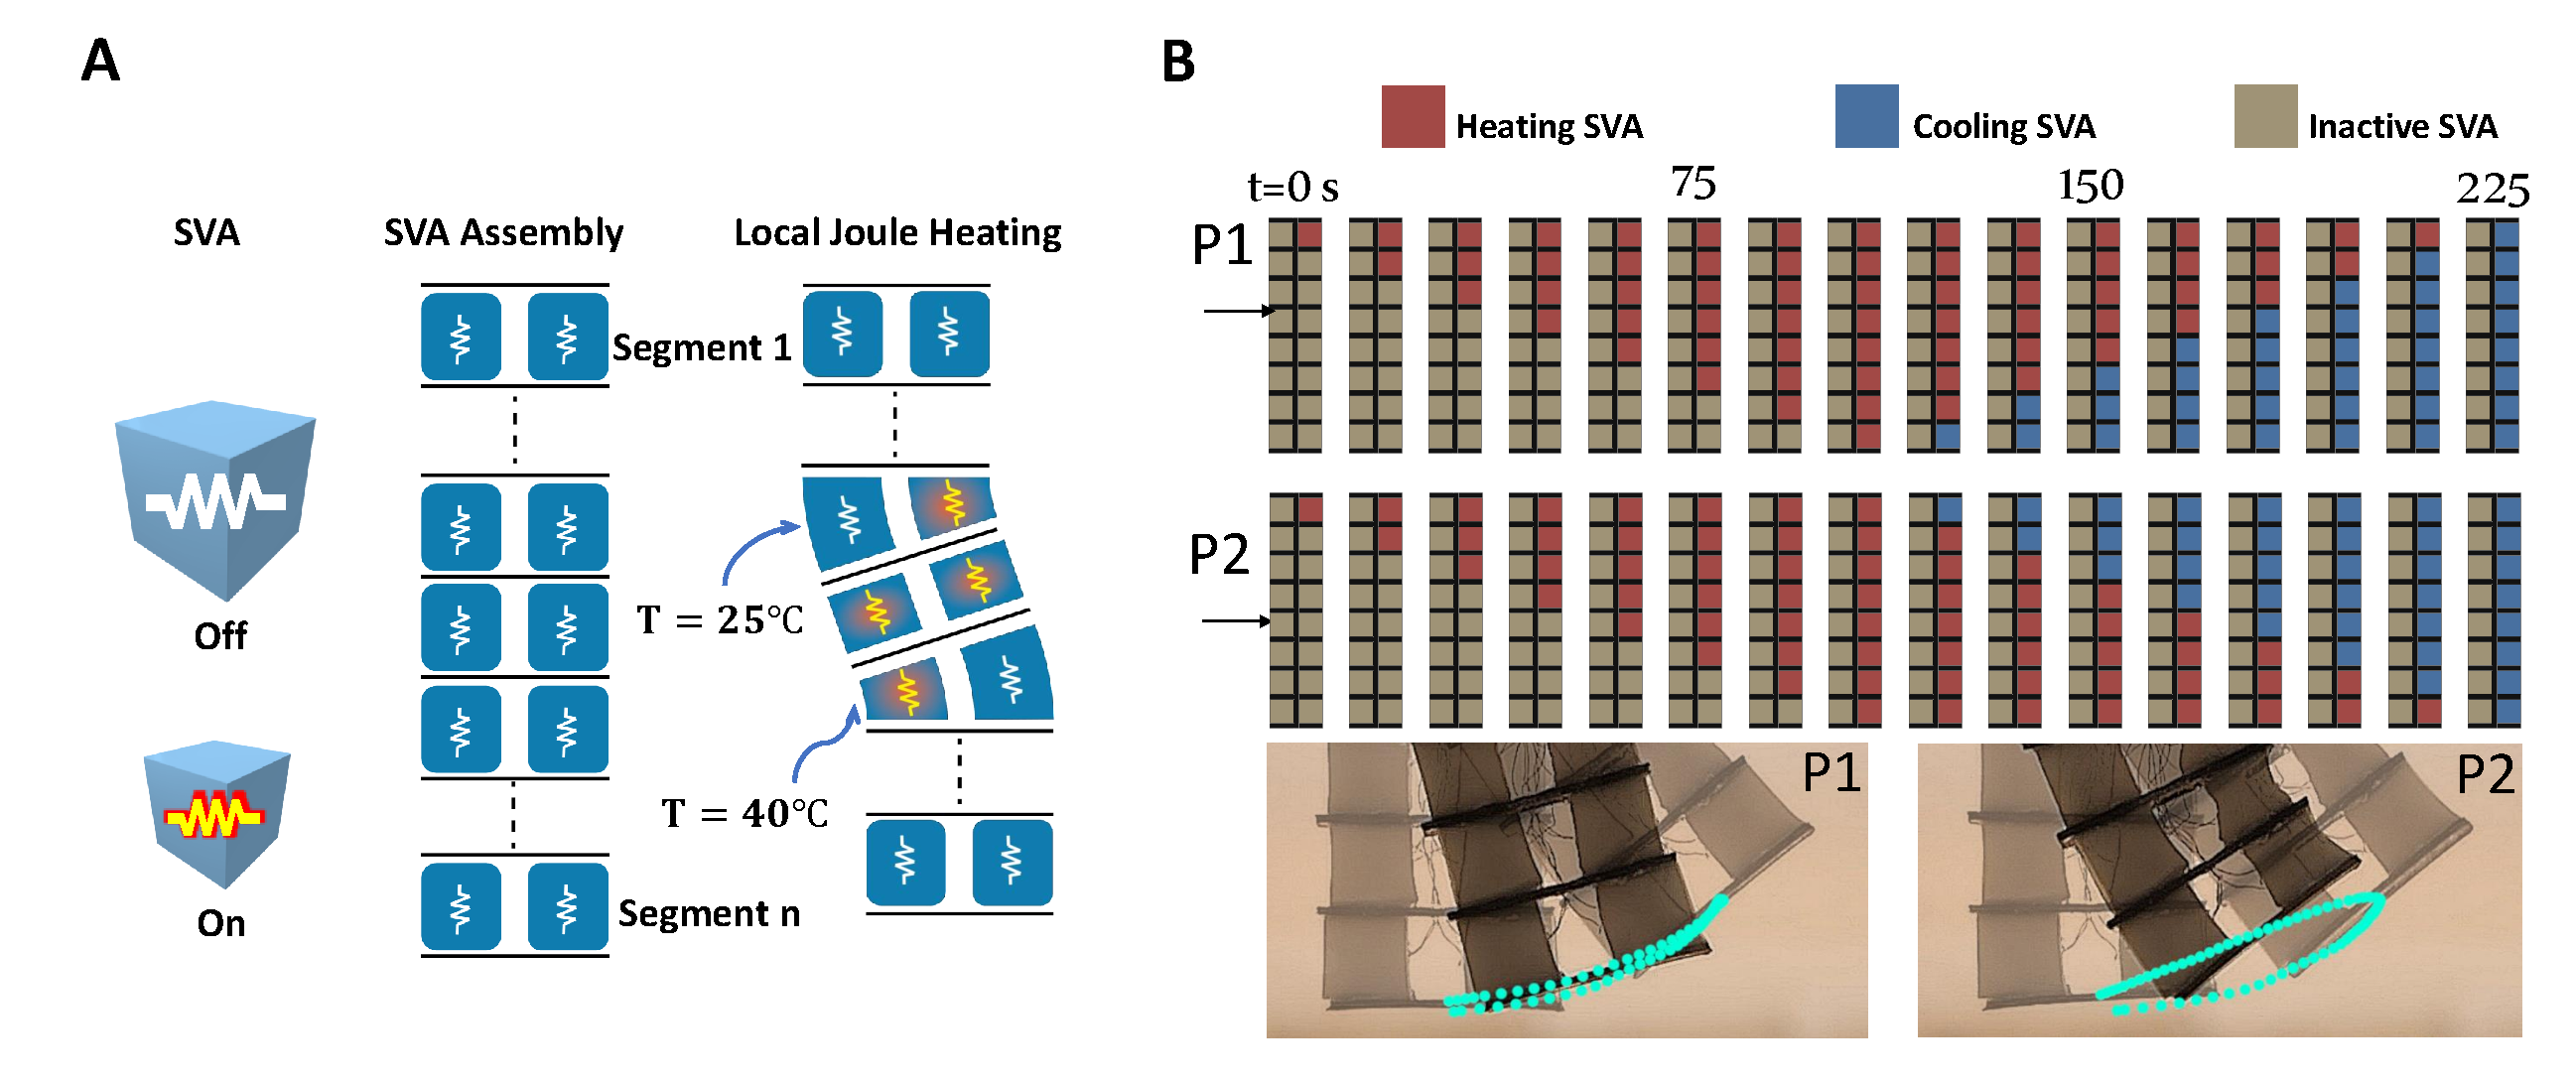
\includegraphics[width=\textwidth]{Fig2.pdf}
      \caption[Trajectory control in a miniature hyper-redundant arm]{A) On and off states of a SVA is shown on the left column. Schematic of an assembly of SVAs is shown on the middle column. Activation of SVAs results in local increase in the temperature which leads to deformations that control the overall motion of the manipulator (right column). B) Sequentially activating SVAs 1 through 8 according to the patterns labeled P1 and P2 results in different trajectories followed by the tip of the manipulator (shown in cyan at the bottom). For details, see Movie S1.}
      \label{fig:treajectory}
   \end{figure*}
	
\section{Soft Voxel Actuators (SVAs)}
A voxel actuator can be made in different shapes and dimensions based on the design requirements. Manufacturing a SVA is performed via a molding process in which a hydrogel precurosor solution is poured into a mold, a Joule heater is inserted in the mold and then the solution is polymerized with a UV LED. Surface  mount  resistors  (10\,ohm  SMD  resistor  0805) were chosen as the heating elements. For the construction of the hyper-redundant manipulator, the voxels are made as cubes of 4.5$\times$4.5$\times$4.5\,mm$^3$ as shown in Fig.~\ref{fig:treajectory}A. In case of the untethered walking robot, voxels of 8$\times$4.5$\times$3\,mm$^3$ are used. Details of hydrogel synthesis, material characterization and SVA manufacturing are discussed in \cite{Khodambashi2021}.

\section{Results}
Hydrogels expand and contract based on the diffusion of water into and out of their structure when the temperature is passed their critical transition temperature -- which is around 32\textsuperscript{o} C in case of PNIPAAm hydrogels. Therefore, all the experiments are performed in a water bath. Fig.~\ref{fig:treajectory}A shows a schematic of a SVA. When the embedded Joule heater is turned on, the temperature increases and the volume of the hydrogel is decreased. When the heater is turned off the SVA cools down and its volume increases. We have shown that a SVA can produce a force of 0.12\,N which is equivalent to a weight of nearly 12\,g. This is 120 times its own weight \cite{Khodambashi2021}. To demonstrate how SVAs support the development of miniature and untethered soft robots, we describe two different robotic platforms in the following sections. 
\subsection{Case Study I: Miniature Hyper-redundant Soft Robotic Arm}
The structure shown in Fig.~\ref{fig:concept}A was assembled using 16 SVA units. The SVAs are connected together using a 0.1 mm thick 3D printed PLA sheets. Dynamic on-demand shape changes are achieved through time-varying activation of SVAs.
As demonstrated in Fig.~\ref{fig:treajectory}B, the choice of SVA actuation pattern can influence the end-effector trajectory of the manipulator. In this experiment, SVAs 1 thorough 8 are activated according to patterns denoted by P1 and P2. Movie S1 shows the resulting trajectories for P1 and P2.
% in \subfigref{fig:4}{D}. 
Each SVA is activated with maximum voltage (3.7\,V) for 15\,s before the next SVA is activated.
The demonstrated miniaturized continuum manipulator with 16 degrees of freedom in a $40\times11\times5$\,mm$^3$ footprint represents the highest reported electrically-addressable number of DOFs in a soft manipulator of these dimensions. 
\subsection{Case Study II: Untethered Miniature Underwater Walking Robot} 
\begin{figure*}[!t]
      \centering
      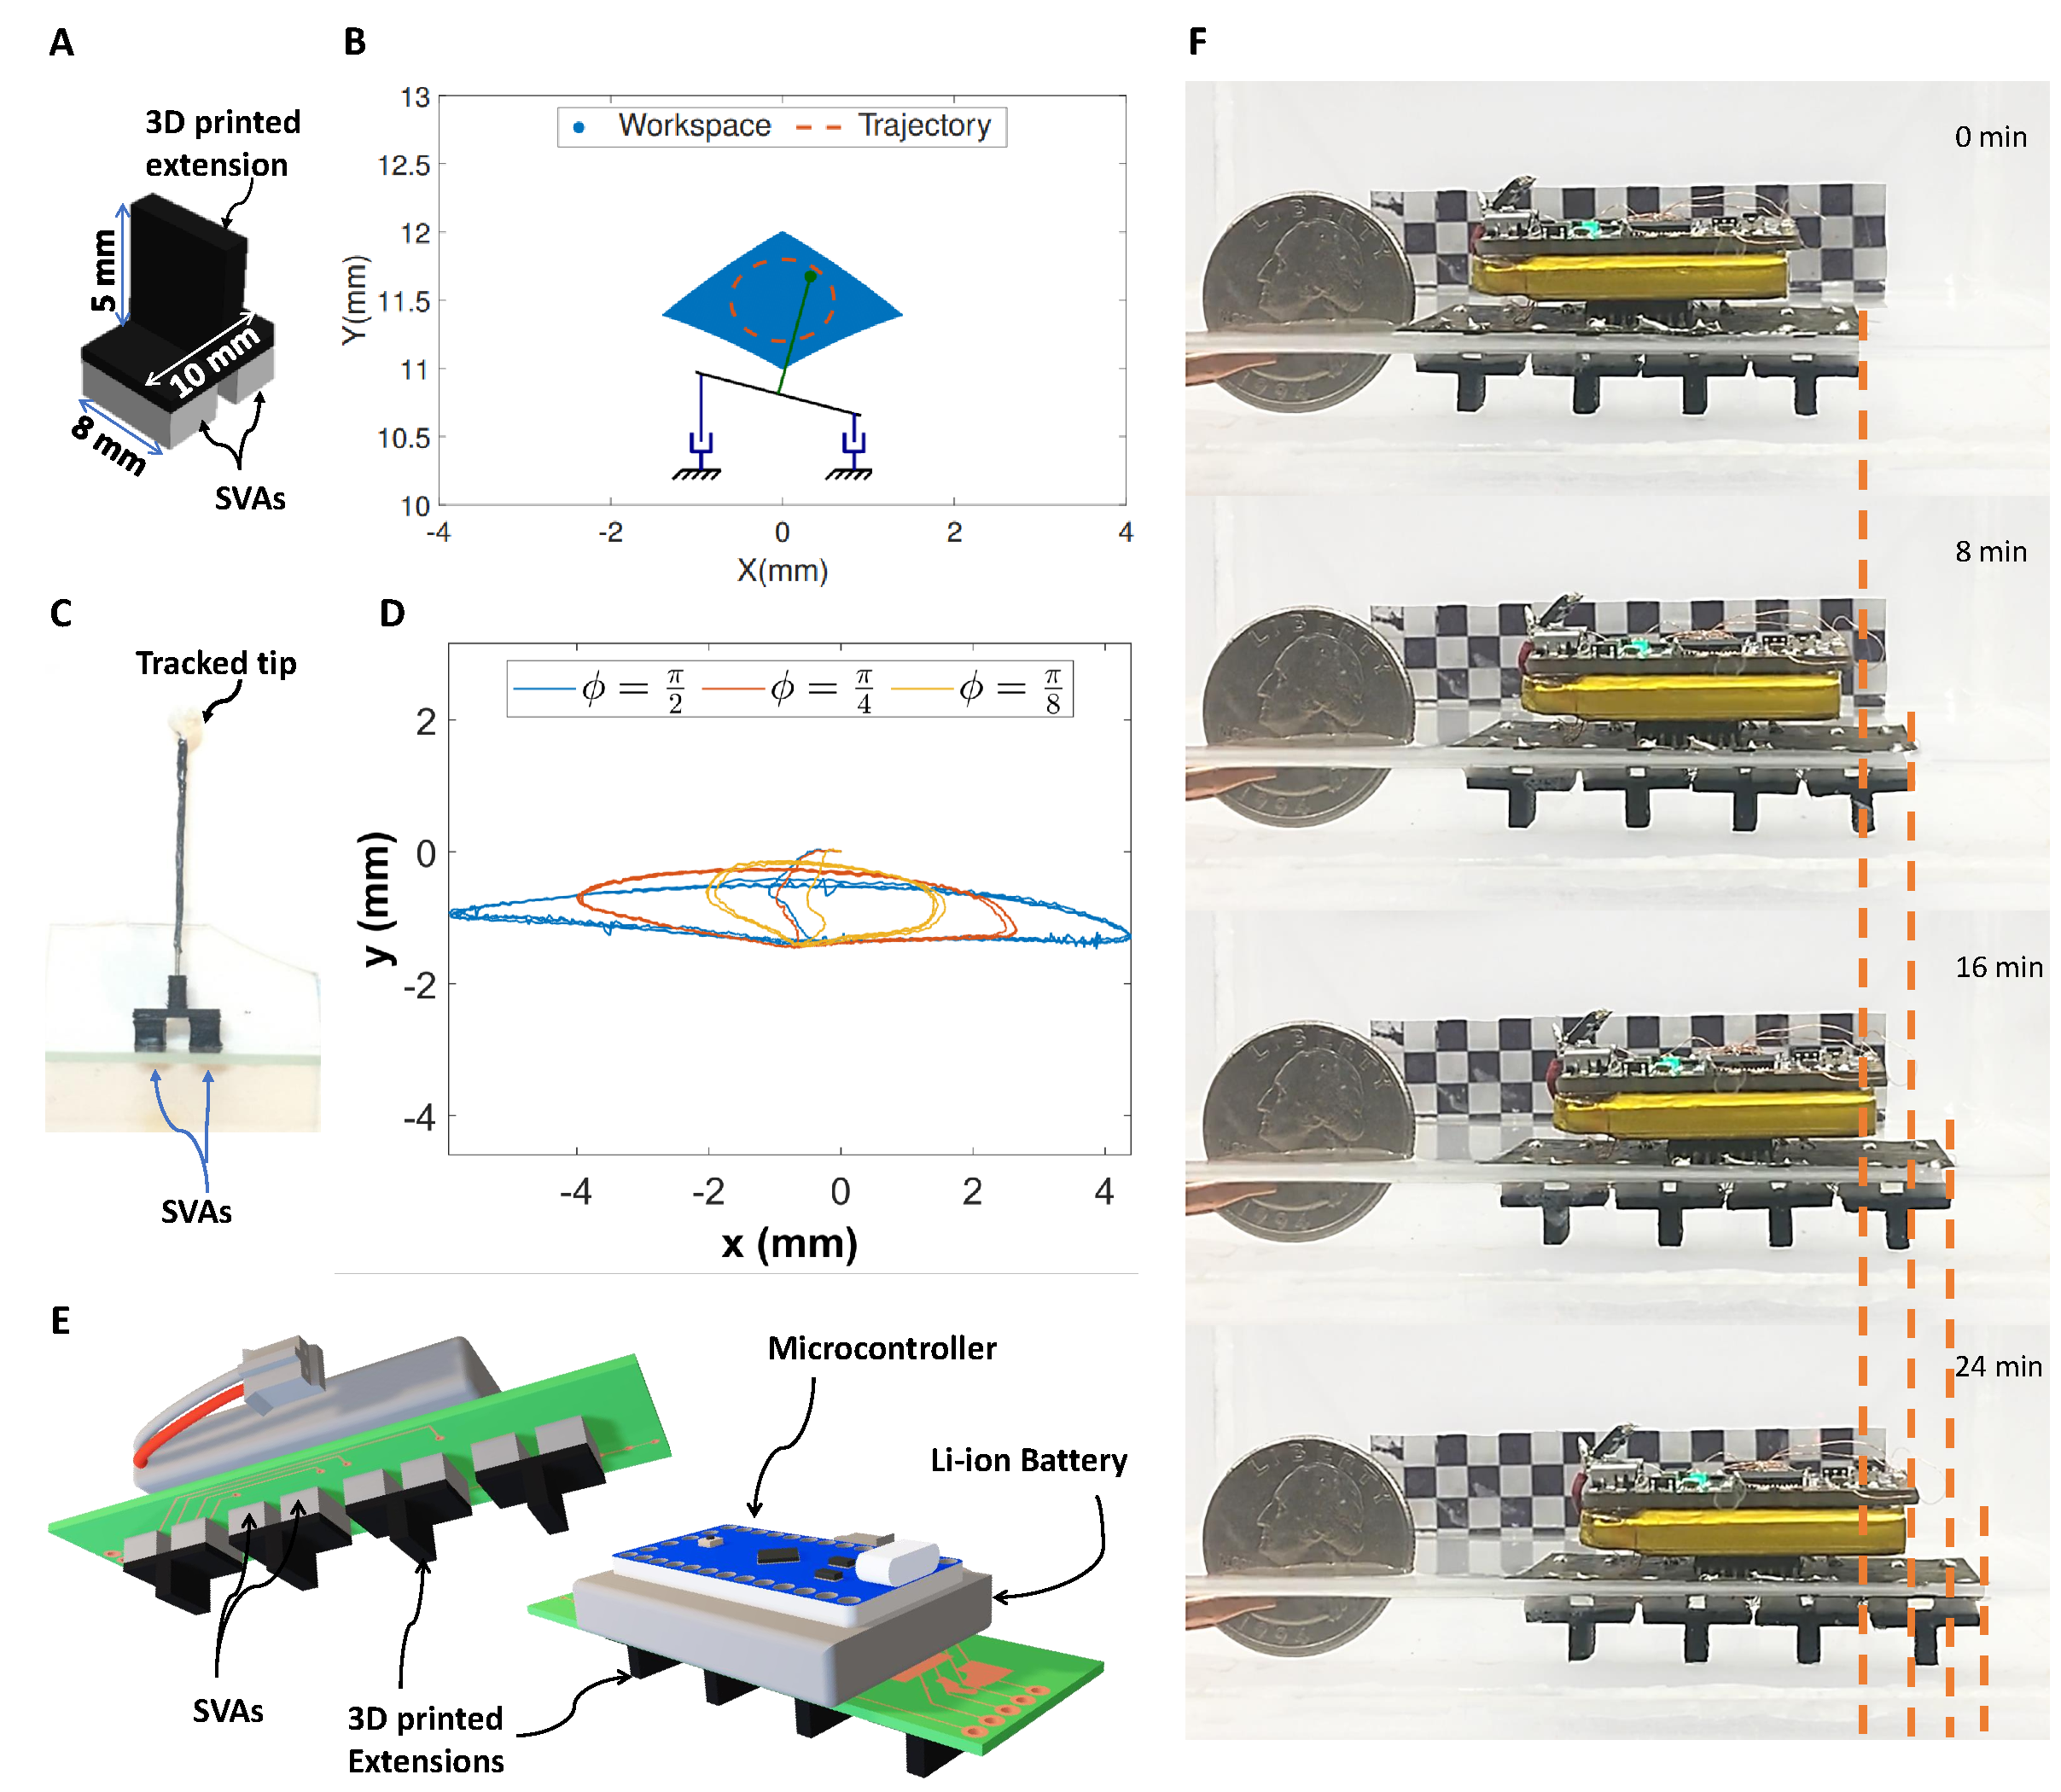
\includegraphics[width=1\textwidth]{Fig3.pdf}
      \caption[Design and evaluation of untethered miniature underwater walking robot]{A) A two degrees of freedom manipulator using two SVAs and a 3D printed extension. B) The workspace of the tip of this manipulator. C) A needle is attached to the tip of the 3D printed extension to amplify the movement of the tip. D) Different trajectories of the tip of the needle as a function of phase shift in the sinusoidal excitation voltages. E) A microcontroller board and a lithium ion battery is added to the system to make an untethered robot. F) Time-lapse of the movement of the miniature underwater walking robot (see Movie S1 for details).}
      \label{fig:untethered_podia}
\end{figure*}
The robot shown in Fig.~\ref{fig:concept}B has four legs. Each leg is a two DOF manipulator composed of 
% To demonstrate the above mentioned features, we have developed a manipulator using 
two SVAs and a 3D printed extension as shown in Fig.~\ref{fig:untethered_podia}A. The workspace of the tip of this manipulator is plotted in Fig.~\ref{fig:untethered_podia}B. To amplify the movement of the tip and measure it more precisely, a needle is attached to the tip of the 3D printed extension. A spherical marker is attached to the end of the needle and functions as a marker for tracking using a camera (Fig.~\ref{fig:untethered_podia}C). The needle is only attached for recording the trajectories and was not present in the final robot prototype. We have created circular and oval trajectories using sine wave voltages as input to the SVAs. Each SVA is actuated using a sine wave with a phase shift with respect to other SVA. As the phase shift between the two SVAs in a manipulator is varied, the shape of the trajectory changes. Fig.~\ref{fig:untethered_podia}D shows different trajectories of the tip of the needle as a function of phase shift in the sinusoidal excitation voltages. To create an untethered walking robot, four manipulators discussed above are assembled in an array. The array is attached to a microcontroller board (Adafruit Itsy Bitsy M0) and a lithium ion battery is added to the system as shown in as shown in Fig.~\ref{fig:untethered_podia}E. The movement of the miniature underwater walking robot is shown as a time-lapse in Fig.~\ref{fig:untethered_podia}F and also can be seen in details in Movie S1.
\subsection{Comparing Actuation of SVAs using Electreical and Light Signals}
Hydrogels can be made to respond to different stimuli such as PH, Light or heat. On-demand shape changes are achieved using light as a control signal~\cite{Wang2015b} In case of temperature responsive hydrogels such as the one presented in this work, any stimulus that can change the temperature of the gel could be used for actuation. Therefore, addition of light absorbing agents that can convert light energy to heat can result in a light responsive hydrogel. Gold nanoparticles are among the highly used light absorbing agents. Under illumination at their plasmonic resonance wavelength, they can turn incident light into efficient nano sources of heat remotely controllable by light. One such light responsive hydrogel is previously demonstrated in {Zhao, Yusen, et al. "Soft phototactic swimmer based on self-sustained hydrogel oscillator." Science Robotics 4.33 (2019).}
\begin{figure*}[!th]
      \centering
      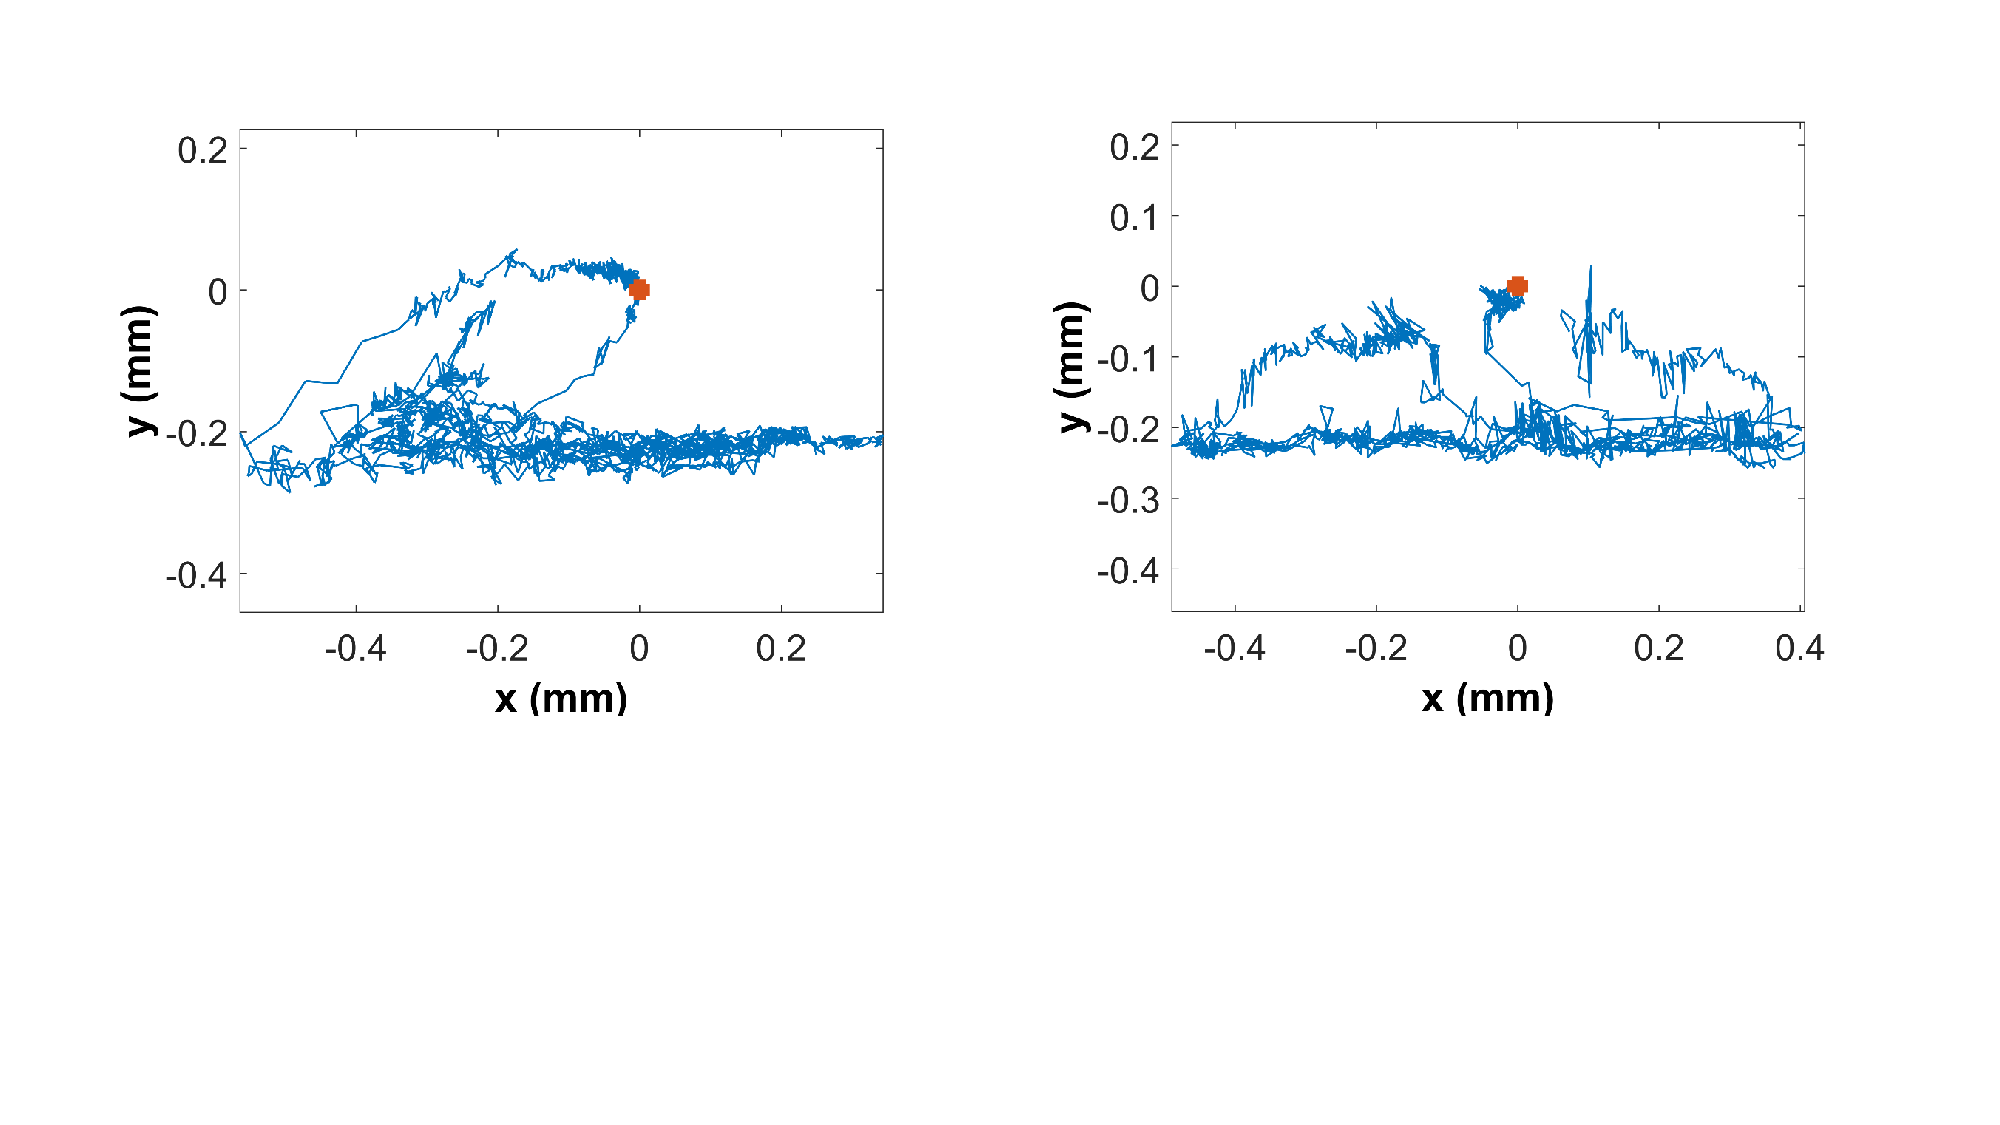
\includegraphics[width=1\textwidth]{Fig4.pdf}
      \caption[Trajectories using a light responding hydrogel]{Trajectories produced using a light responding hydrogel. Light responding SVAs are activated using a laser source pointed manually by a human operator.}
      \label{fig:laser}
\end{figure*}
Here, to show some possibilities, polypyrrole as a light absorbing material is used to create SVAs that respond to a light beam. Using this light-responsive gel, a manipulator similar to Fig.~\ref{fig:untethered_podia}C  is built using two SVAs. As before, the goal is to move the tip of the mechanism in an oval loop. The trajectory of the tip is recorded using a camera and is shown in Figure~\ref{fig:laser}. It is clearly seen that using light as a control signal results in a random trajectory which is far from the desired one. This is because the laser beam is manually shined on the SVAs. Even if a motorized mechanism is used to shine the light, it only complicates the system and diverge it from being usable as a mobile robotic platform.  In contrast, the electric stimulation results in a much smoother trajectory which is repeatable over many cycles. It is also possible to program the desired trajectory by varying the activation voltage of SVAs. In this experiment, two sinusoidal voltages are used that have a phase shift which result in circular motion of the tip as discussed before. Animals use electric signals for activation of their muscles and the analogy of SVAs to motor units was the source of inspiration to stay with electric signals as opposed to other activation modes so that the resulting mechanisms are more independent of the environment and are more easily controlled. 



\section{Conclusions}
We have shown that the voxel-based design and manufacturing strategy, combined with an electrically addressable smart material, can lead to the creation of miniaturized soft robots with a high number of DOFs. These robots can be used for tasks in which redundancy is needed for example to handle continuously changing tasks in unstructured environments. This has been demonstrated through a miniaturized hyper-redundant soft robot with 16 SVA units.
SVAs can be easily integrated into robotic systems. They help greatly reduce the size of the robots. In addition, sice the SVAs are electrically controlled, they can be connected directly to small footprint microcontrollers and other electronics. The electronics and power supply can be embedded in the robot  and cut the tether from the entire system. We have demonstrated this through a miniature underwater walking robot that do not rely on external signals or power which can be beneficial in applications such as under water data collection and ocean monitoring. The SVAs introduced in this paper are the first demonstration of active, soft voxels that are made of stimuli-responsive materials. Using SVAs as building blocks offers higher number of design parameters, namely, the configuration of the SVAs, the material properties of each SVA, and the activation voltage of each SVA. Multi-objective optimization can be used in future to optimize this rich set of design parameters to build structures that have higher force production capacity and %higher 
energy efficiency.
% miniature and micro-scale soft actuators have matured more slowly than their  macro-scale counterparts. 

